% AR-521 end-semester project report. Compile on Overleaf (pdfLaTeX + BibTeX).
% Upload this folder together with ../results/figures and ../results/tables.
\documentclass[11pt,a4paper]{article}
\usepackage[margin=2.2cm]{geometry}
\usepackage{amsmath,amssymb,bm}
\usepackage{graphicx,booktabs,siunitx,hyperref,cleveref,caption,subcaption}
\usepackage[numbers]{natbib}
\usepackage{float}
\graphicspath{{figures/}{../results/figures/}}
\newcommand{\R}{\mathbb{R}}
\newcommand{\wrap}{\operatorname{wrap}}

\title{Trajectory Tracking Control of a TurtleBot3 using\\Nonlinear Model Predictive Control with Obstacle Avoidance}
\author{Rishang Yadav (B23173)\\AR-521 Control for Robotic Systems --- End-Semester Project, IIT Mandi}
\date{\today}

\begin{document}
\maketitle

\begin{abstract}
We design, implement and evaluate a nonlinear model predictive controller (NMPC) for trajectory tracking of a TurtleBot3 Burger differential-drive robot with on-line obstacle avoidance from 2D LiDAR. The NMPC uses a multiple-shooting transcription of the unicycle model, the robot's coupled wheel-speed limits, rate limits and discrete-time control-barrier-function (CBF) obstacle constraints with exact-penalty slacks, solved with IPOPT at \SI{10}{Hz}. The controller runs unchanged in a kinematic simulator, in Gazebo and on hardware through ROS~2. We compare it against Kanayama's controller, the Samson law (equivalent to kinematic backstepping) and a kinematic sliding-mode controller, all subject to identical saturation, sampling, state feedback and tuning budget, in a paired Monte Carlo study over randomized trajectories, initial poses and obstacles, with robustness sweeps over delay, noise and model mismatch. With obstacles, NMPC reaches the goal in 100\% of 60 LiDAR-perceived scenarios without collision, whereas the same baselines behind a CBF-QP safety filter are collision-free but deadlock in 43--100\% of runs; obstacle-free, NMPC is significantly the most accurate on references with varying curvature or stops, while well-tuned static laws match or beat it on constant-curvature references and under unmodelled wheel asymmetry. Warm-started solves take a median of \SI{10}{ms} (p99 \SI{21}{ms}) at $N=20$ with obstacle constraints.
\end{abstract}

\section{Introduction}
% Problem statement items -> where they are addressed:
% initial & goal positions vary -> random offsets + point-to-point (Sec. 6)
% random & desired trajectories -> flatness-based families + random splines (Sec. 3)
% obstacle avoidance -> CBF constraints + LiDAR pipeline (Sec. 5)
% modelling & formulation -> Sec. 2, 4
% sensor acquisition & feedback -> Sec. 5-6 (odometry, LiDAR, delay compensation)
Contributions: (i) an NMPC formulation that respects the Burger's true (coupled) actuator limits and encodes obstacles as discrete-time CBF constraints~\cite{zeng2021mpccbf}; (ii) a sim--Gazebo--hardware pipeline sharing one tested core; (iii) a fair, statistically tested comparison against three classical nonlinear tracking laws~\cite{kanayama1990,samson1995,elyoussef2014}.

\section{Modelling}
\subsection{Kinematics}
With pose $\bm{x}=[x,\,y,\,\theta]^\top$ in the \texttt{odom} frame and body-frame input $\bm{u}=[v,\,\omega]^\top$,
\begin{equation}
\dot{\bm{x}} = f(\bm{x},\bm{u}) = \begin{bmatrix} v\cos\theta \\ v\sin\theta \\ \omega \end{bmatrix}. \label{eq:unicycle}
\end{equation}
The model is nonholonomic ($\dot x\sin\theta-\dot y\cos\theta=0$); its linearization about a rest point is not stabilizable by smooth static feedback (Brockett), which motivates time-varying references and nonlinear control.

\subsection{Discretization}
Zero-order hold with $\Delta t=\SI{0.1}{s}$ and one classical RK4 step, $\bm{x}_{k+1}=F(\bm{x}_k,\bm{u}_k)$. At $v\le\SI{0.22}{m/s}$ the robot moves at most \SI{2.2}{cm} per step.

\subsection{Actuator limits}
With wheel separation $L=\SI{0.160}{m}$, wheel rim speeds are $v_{R,L}=v\pm\tfrac{L}{2}\omega$ and are limited by $v_w^{\max}=\SI{0.22}{m/s}$, giving the \emph{wheel diamond}
\begin{equation}
|v| + \tfrac{L}{2}|\omega| \le v_w^{\max}, \qquad |v|\le 0.22,\ |\omega|\le 2.84, \label{eq:diamond}
\end{equation}
which is the binding constraint (e.g.\ at $v=\SI{0.15}{m/s}$, $|\omega|\le\SI{0.875}{rad/s}$). We add rate limits $|\Delta v|\le a_{\max}\Delta t$, $|\Delta\omega|\le\alpha_{\max}\Delta t$ with $a_{\max}=\SI{0.5}{m/s^2}$, $\alpha_{\max}=\SI{3}{rad/s^2}$ (engineering choices; the driver applies no acceleration profile). The same saturation block (rate $\to$ box $\to$ curvature-preserving diamond scaling) is applied to every controller.

\section{Reference generation}
The position $(x,y)$ is a flat output of \eqref{eq:unicycle}~\cite{oriolo2002}: for any $C^2$ path,
\begin{equation}
\theta_r=\operatorname{atan2}(\dot y_r,\dot x_r),\quad v_r=\sqrt{\dot x_r^2+\dot y_r^2},\quad \omega_r=\frac{\dot x_r\ddot y_r-\dot y_r\ddot x_r}{\dot x_r^2+\dot y_r^2}.
\end{equation}
Families: circle, Gerono lemniscate (figure-8), sinusoid, a time-scaled Lissajous curve, \emph{random splines} (5--8 seeded waypoints in a \SI{3x3}{m} arena, natural cubic spline on chord length, curvature-limited) and \emph{point-to-point} (rest-to-rest cubic B\'ezier between random start/goal poses). Path-based references are time-parameterized with $v(s)=\min\{0.8v_{\max},\,0.8\omega_{\max}/|\kappa|,\,0.8v_w^{\max}/(1+\tfrac L2|\kappa|)\}$ and forward/backward acceleration passes, leaving 20\% feedback headroom.

\section{Controllers}
\subsection{Tracking error}
All controllers use the robot-frame error~\cite{kanayama1990}
$\bm{e}=[e_x,e_y,e_\theta]^\top$, $[e_x,e_y]^\top=R(\theta)^\top(\bm p_r-\bm p)$, $e_\theta=\wrap(\theta_r-\theta)$, with dynamics
$\dot e_x=\omega e_y-v+v_r\cos e_\theta$, $\dot e_y=-\omega e_x+v_r\sin e_\theta$, $\dot e_\theta=\omega_r-\omega$.

\subsection{Nonlinear MPC}
At each sample, with measured (or delay-compensated) state $\hat{\bm x}$, previous input $\bm u_{-1}$ and obstacle circles $\{(\bm c_j,r_j)\}_{j=1}^{M}$ (inflated by robot radius and margin):
\begin{align}
\min_{\bm X,\bm U,\bm S}\ & \sum_{k=0}^{N-1}\Big[\|\bm p_k-\bm p_k^r\|^2_{Q}+2q_\theta(1-\cos(\theta_k-\theta^r_k))+\|\bm u_k-\bm u^r_k\|^2_R+\|\bm u_k-\bm u_{k-1}\|^2_{S}\Big] \nonumber\\
&+\|\bm p_N-\bm p_N^r\|^2_{P}+2p_\theta(1-\cos(\theta_N-\theta^r_N)) + \rho\,\mathbf{1}^\top\bm S \label{eq:cost}\\
\text{s.t.}\ & \bm x_0=\hat{\bm x},\quad \bm x_{k+1}=F(\bm x_k,\bm u_k),\quad \eqref{eq:diamond},\ \text{rate limits},\nonumber\\
& h_j(\bm x_{k+1})\ge(1-\gamma)\,h_j(\bm x_k)-s_{j,k},\quad s_{j,k}\ge0,\quad k=0,\dots,N-1,\ j=1,\dots,M, \label{eq:cbf}
\end{align}
with $h_j(\bm x)=\|\bm p+\ell[\cos\theta,\sin\theta]^\top-\bm c_j\|^2-r_j^2$. Design choices and their reasons:
\begin{itemize}
\item $1-\cos$ heading cost: smooth, $2\pi$-periodic, no wrap discontinuity.
\item Penalizing $\bm u-\bm u^r$ (not $\bm u$): zero cost for following the flat feed-forward.
\item Look-ahead $\ell=\SI{5}{cm}$: puts $\theta$ (hence $\omega$) into $h$; otherwise one Euler step of $h$ depends on $v$ only and the CBF can only brake, not steer.
\item Discrete CBF (\ref{eq:cbf}) vs distance constraint $h_j(\bm x_k)\ge0$: the CBF bounds the decay of the safety margin by $(1-\gamma)$ per step and acts before contact; distance constraints are inactive until the predicted trajectory touches the obstacle~\cite{zeng2021mpccbf}.
\item Exact L1 penalty $\rho=10^4$: equals the hard-constrained solution whenever that is feasible, but never makes the NLP infeasible (sensor noise, newly seen obstacles).
\item Terminal cost $P=10Q$ only. Stability results for receding-horizon unicycle tracking use a terminal penalty \emph{and} terminal set~\cite{gu2006}; we omit the set to preserve feasibility near obstacles (as in~\cite{salimi2021}) and verify convergence empirically.
\end{itemize}
Implementation: CasADi SX, multiple shooting ($3(N{+}1)+2N+MN$ variables), IPOPT with warm start from the shifted previous primal--dual solution; obstacle slots are a fixed $3\times M$ parameter padded with far-away dummies so the NLP is built once. On solver failure the next input of the previous plan is applied (up to 3 times), then the robot brakes.

\subsection{Baselines}
\paragraph{Kanayama~\cite{kanayama1990}.} $v=v_r\cos e_\theta+k_xe_x$, $\omega=\omega_r+v_r(k_ye_y+k_\theta\sin e_\theta)$, $k_\theta=2\sqrt{k_y}$. With $V=\tfrac12(e_x^2+e_y^2)+(1-\cos e_\theta)/k_y$: $\dot V=-k_xe_x^2-\tfrac{v_rk_\theta}{k_y}\sin^2e_\theta\le0$ (needs $v_r>0$).
\paragraph{Samson / kinematic backstepping~\cite{samson1995,jiang1997}.} $v=v_r\cos e_\theta+k_1e_x$, $\omega=\omega_r+k_2v_r\operatorname{sinc}(e_\theta)e_y+k_3e_\theta$, $k_1=k_3=2\zeta\sqrt{\omega_r^2+bv_r^2}$, $k_2=b$; $V=\tfrac{k_2}{2}(e_x^2+e_y^2)+\tfrac12e_\theta^2$, $\dot V=-k_1k_2e_x^2-k_3e_\theta^2$. At the kinematic level backstepping reduces to this law, so we count it once.
\paragraph{Kinematic SMC~\cite{elyoussef2014}.} Surfaces $s_v=k_1e_x$, $s_\omega=k_2e_y+k_3\sin(e_\theta/2)$, reaching law $\dot s=-K\operatorname{sat}(s/\phi)-Ps$, giving
$\omega=\big[k_2v_r\sin e_\theta+\tfrac{k_3}{2}\cos\tfrac{e_\theta}{2}\,\omega_r+K_\omega\operatorname{sat}(s_\omega/\phi)+P_\omega s_\omega\big]/\big[k_2e_x+\tfrac{k_3}{2}\cos\tfrac{e_\theta}{2}\big]$ and
$v=\omega e_y+v_r\cos e_\theta+[K_v\operatorname{sat}(s_v/\phi)+P_vs_v]/k_1$ (denominator guarded). The torque-level SMC of~\cite{yang1999} is unnecessary for a velocity-commanded robot.
\paragraph{Obstacles for baselines.} Classical trackers have no obstacle model, so in obstacle runs each is wrapped in a CBF-QP safety filter with the same barrier: $\min_{\bm u}\|\bm u-\bm u_{\text{nom}}\|_W^2$ s.t.\ $\dot h_j\ge-\alpha h_j$, box and diamond limits.

\section{System architecture, sensing and feedback}
% Figure: node graph (PLAN.md ASCII -> draw.io / TikZ)
\begin{itemize}
\item \textbf{State feedback:} \texttt{/odom} (wheel encoders, IMU heading fusion inside \texttt{turtlebot3\_node}; $\approx$\SI{20}{Hz}).
\item \textbf{Obstacle sensing:} \texttt{/scan} (LDS, \SI{5}{Hz}, 360 beams) $\to$ invalid-beam masking (0 and $\infty$) $\to$ adaptive-breakpoint segmentation~\cite{borges2004} with wrap-around merge $\to$ chunking of long segments $\to$ Kåsa least-squares circle fit $\to$ tf2 transform to \texttt{odom} at the scan timestamp $\to$ inflation $\to$ $K$ nearest.
\item \textbf{Delay compensation:} the controller integrates \eqref{eq:unicycle} from the odometry stamp to $t_{\text{now}}+\tau$ through the commands already sent, and plans from that predicted state.
\item \textbf{Safety layers:} stale-odometry/obstacle watchdogs, forward-sector proximity stop, \texttt{/estop}, and an on-robot \texttt{cmd\_vel} relay with a \SI{0.3}{s} timeout (the TurtleBot3 driver has none).
\end{itemize}

\section{Experimental protocol}
Three tiers: (1) kinematic simulator --- statistical bulk; (2) Gazebo with encoder odometry and p3d ground truth --- confirmation and obstacle scenarios; (3) hardware --- demonstration runs with taped ground truth. Paired design: seed $s$ fixes the reference (random families), initial offset ($\pm\SI{0.2}{m}$, $\pm\pi/6$), noise sequence and obstacles; every controller sees the same seed ($M=30$ per cell). Gains of \emph{all} controllers were tuned with the same budget (24 grid points) on held-out seeds and frozen. Metrics: RMSE / max position error over $t\in[\SI{5}{s},T_{\text{ref}}]$, heading RMSE, IAE, control effort and smoothness, saturation \%, min clearance, collisions, success, and solve-time statistics. Statistics: median [IQR], 95\% bootstrap CI, paired Wilcoxon signed-rank tests with Holm correction.

\section{Results}
All tables and figures are generated by \texttt{experiments/analyze.py} from the raw episode logs; Table~\ref{tab:gains} lists the frozen gains every controller used.
\begin{table}[!htbp]
\centering\small
\caption{Frozen gains after equal-budget tuning (24 candidates per controller, held-out seeds).}\label{tab:gains}
\begin{adjustbox}{max width=\linewidth}
\begin{tabular}{llr}
\toprule
controller & tuned parameters & tuning RMSE [mm] \\
\midrule
Kanayama & $k_x=2$, $k_y=200$ & 1.73 \\
Samson / backstepping & $\zeta=1.2$, $b=120$ & 2.30 \\
Kinematic SMC & $k_2=8$, $k_3=2$, $\phi=0.02$ & 0.65 \\
NMPC & $q_{xy}=30$, $q_\theta=0.5$, $r_v=0.1$, $s_v=0.3$ & 0.22 \\
\bottomrule
\end{tabular}
\end{adjustbox}
\end{table}


\subsection{Obstacle-free tracking}
Table~\ref{tab:tracking} and Fig.~\ref{fig:trackbox}. All controllers track every family to sub-centimetre accuracy in the nominal kinematic setting, so differences are in tenths of a millimetre. NMPC is significantly best on references with varying curvature or stops (Lissajous, random splines, point-to-point), where its horizon previews upcoming curvature and decelerations. On constant- or slowly-varying-curvature references a well-tuned static law is as good or better (Kanayama on the circle, SMC on the figure-8 and sinusoid).
\begin{table}[t]
\centering\small
\caption{Obstacle-free tracking: median position RMSE and median max error over 30 paired seeds (mm, $t\in[5\,\mathrm{s},T_{\mathrm{ref}}]$). Best in bold.}\label{tab:tracking}
\resizebox{\linewidth}{!}{%
\begin{tabular}{lrrrrrrrr}
\toprule
& \multicolumn{4}{c}{RMSE [mm]} & \multicolumn{4}{c}{max error [mm]} \\
\cmidrule(lr){2-5}\cmidrule(lr){6-9}
family & NMPC & Kanayama & Samson & SMC & NMPC & Kanayama & Samson & SMC \\
\midrule
circle & 0.09$^{\dagger}$ & \textbf{0.01} & 0.22 & 0.06 & 0.94 & \textbf{0.09} & 1.71 & 0.54 \\
figure8 & 0.20$^{\dagger}$ & 0.26 & 0.29 & \textbf{0.10} & 4.48 & \textbf{0.41} & 1.75 & 0.61 \\
sinusoid & 0.50 & 0.74 & 0.78 & \textbf{0.38} & 7.60 & \textbf{1.01} & 3.21 & 2.16 \\
lissajous & \textbf{0.06}$^{*}$ & 0.27 & 1.74 & 0.47 & \textbf{0.94} & 1.65 & 9.79 & 3.40 \\
random spline & \textbf{0.15}$^{*}$ & 0.60 & 0.68 & 0.24 & \textbf{0.62} & 4.88 & 4.41 & 2.18 \\
point to point & \textbf{0.31}$^{*}$ & 1.37 & 1.87 & 0.72 & \textbf{1.05} & 6.02 & 6.70 & 3.97 \\
\bottomrule
\end{tabular}}
\par\smallskip\footnotesize $^{*}$ NMPC significantly better than every baseline; $^{\dagger}$ at least one baseline significantly better than NMPC (paired Wilcoxon signed-rank, Holm-corrected, $p<0.05$).
\end{table}

\begin{figure}[t]\centering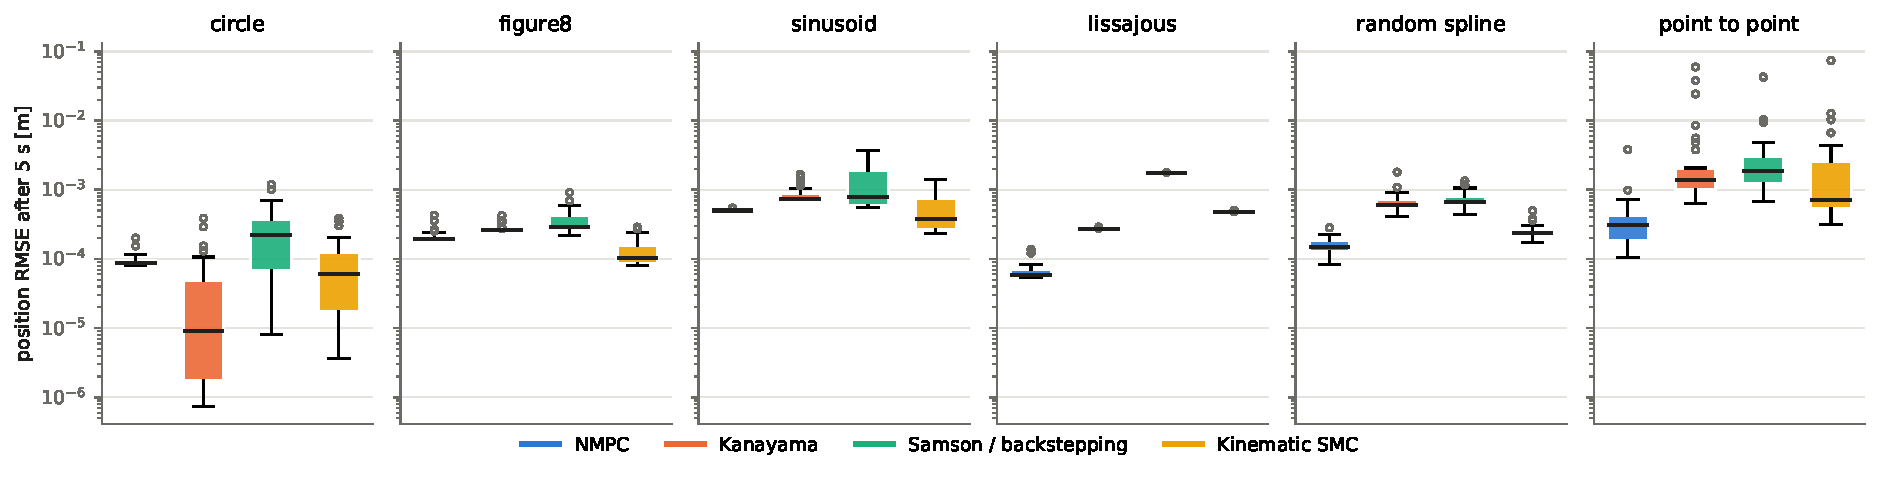
\includegraphics[width=\linewidth]{tracking_rmse_box.pdf}\caption{Position RMSE per reference family over 30 paired seeds (log scale).}\label{fig:trackbox}\end{figure}
\begin{figure}[t]\centering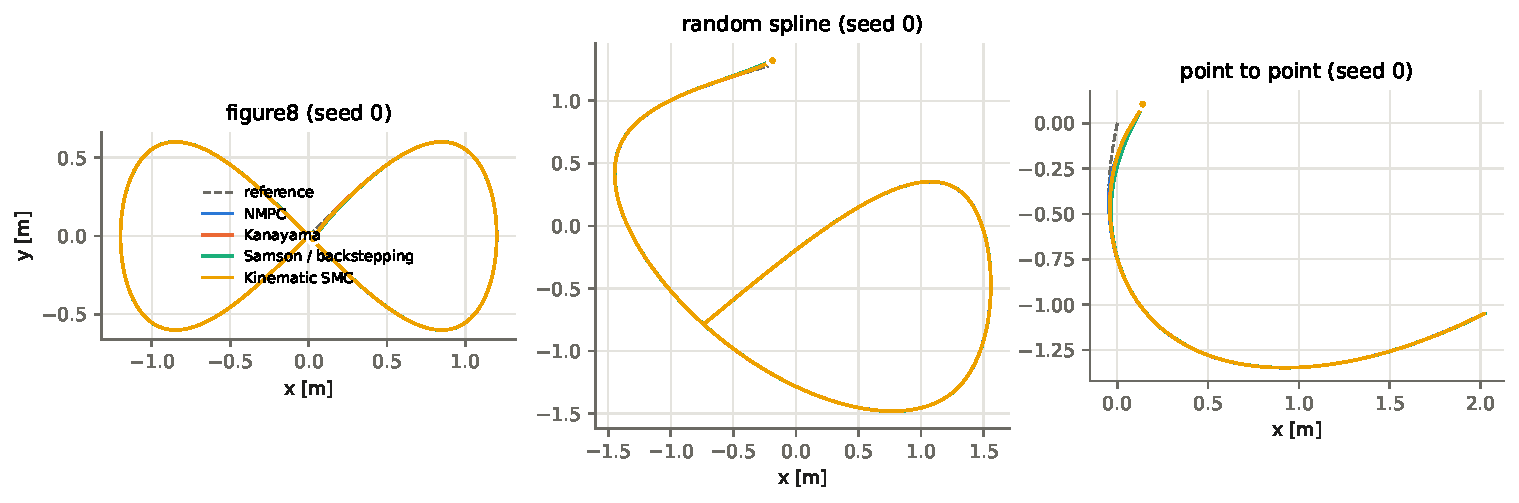
\includegraphics[width=\linewidth]{tracking_xy.pdf}\caption{Example closed-loop trajectories from a random initial offset (seed 0).}\label{fig:trackxy}\end{figure}

\subsection{Robustness}
Table~\ref{tab:robustness}, Fig.~\ref{fig:robust}. Input delay is the dominant failure mode for every controller; the delay-compensated NMPC (forward prediction through committed inputs) is essentially unaffected up to \SI{400}{ms}. NMPC degrades faster than the classical laws under pose noise and asymmetric wheel-radius error (model mismatch it cannot see), where the SMC's matched-disturbance robustness pays off. NMPC is the most robust to large initial offsets because constraints and preview prevent the saturation-induced overshoot of the static laws.
\begin{table}[t]
\centering\small
\caption{Robustness sweeps on random splines: median position RMSE [mm] (30 paired seeds per cell). Perturbations act on the plant only.}\label{tab:robustness}
\resizebox{\linewidth}{!}{%
\begin{tabular}{llrrrrr}
\toprule
perturbation & level & NMPC & Kanayama & Samson & SMC & NMPC + delay comp. \\
\midrule
delay [ms] & 0 & \textbf{0.15} & 0.60 & 0.68 & 0.24 & -- \\
delay [ms] & 100 & 0.60 & 1.55 & 1.40 & 1.90 & \textbf{0.15} \\
delay [ms] & 200 & 1.69 & 16.80 & 2.71 & 7.87 & \textbf{0.16} \\
delay [ms] & 400 & 246.09 & 266.71 & 119.93 & 58.87 & \textbf{0.18} \\
pose noise $\sigma$ [mm] & 0 & \textbf{0.15} & 0.60 & 0.68 & 0.24 & -- \\
pose noise $\sigma$ [mm] & 5 & 3.20 & \textbf{2.37} & 2.98 & 3.72 & -- \\
pose noise $\sigma$ [mm] & 10 & 6.57 & \textbf{4.85} & 5.90 & 7.15 & -- \\
pose noise $\sigma$ [mm] & 20 & 14.06 & \textbf{12.06} & 12.25 & 14.09 & -- \\
wheel radius error [\%] & 0 & \textbf{0.15} & 0.60 & 0.68 & 0.24 & -- \\
wheel radius error [\%] & 5 & 1.83 & 4.35 & 2.06 & \textbf{1.46} & -- \\
wheel radius error [\%] & 10 & 3.46 & 9.20 & 4.24 & \textbf{3.07} & -- \\
wheel asymmetry $\pm$[\%] & 0 & \textbf{0.15} & 0.60 & 0.68 & 0.24 & -- \\
wheel asymmetry $\pm$[\%] & 2 & 2.64 & 1.39 & 2.17 & \textbf{0.39} & -- \\
wheel asymmetry $\pm$[\%] & 5 & 6.59 & 3.16 & 5.17 & \textbf{0.79} & -- \\
initial offset [m] & 0.1 & \textbf{0.14} & 0.58 & 0.64 & 0.23 & -- \\
initial offset [m] & 0.2 & \textbf{0.15} & 0.60 & 0.69 & 0.24 & -- \\
initial offset [m] & 0.4 & \textbf{0.22} & 4.91 & 1.74 & 20.67 & -- \\
\bottomrule
\end{tabular}}
\end{table}

\begin{figure}[t]\centering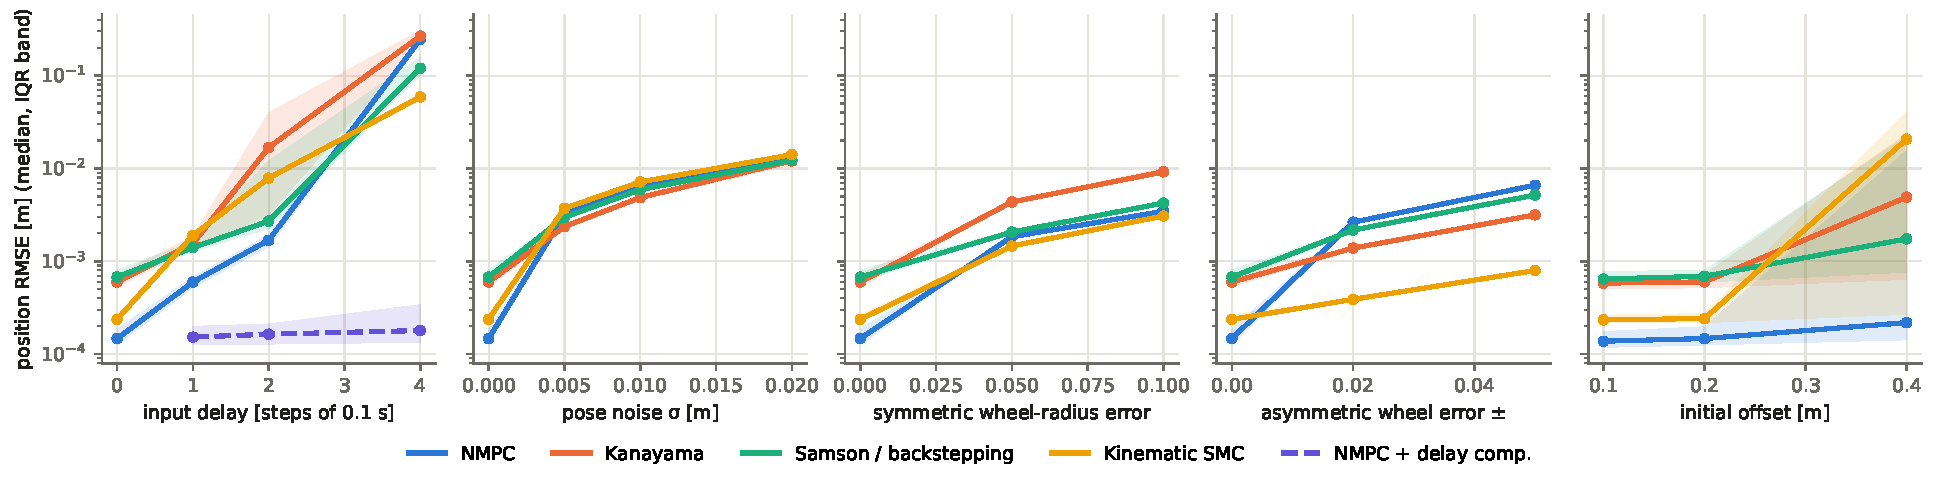
\includegraphics[width=\linewidth]{robustness_degradation.pdf}\caption{Degradation curves: median RMSE with IQR band vs perturbation level (30 paired seeds per point).}\label{fig:robust}\end{figure}

\subsection{Obstacle avoidance}
Table~\ref{tab:obstacles}, Figs.~\ref{fig:obsclear}--\ref{fig:obsxy}. With identical LiDAR perception and the same barrier function, every NMPC variant reaches the goal in all 60 scenarios without collision, whereas the CBF-QP-filtered baselines are \emph{safe} (no collisions) but deadlock in front of obstacles in 43--100\% of runs: the filter is myopic and only removes the unsafe component of the nominal command, while the NMPC re-plans around the obstacle over its horizon. The advantage therefore comes from prediction and constraints, not from better tracking.
\begin{table}[t]
\centering\small
\caption{Obstacle scenarios (2 LiDAR-perceived obstacles, 30 paired seeds per family). Clearance is the median minimum distance between robot footprint and true obstacle boundary.}\label{tab:obstacles}
\resizebox{\linewidth}{!}{%
\begin{tabular}{lrrrrrr}
\toprule
& \multicolumn{3}{c}{random spline} & \multicolumn{3}{c}{point-to-point} \\
\cmidrule(lr){2-4}\cmidrule(lr){5-7}
controller & success [\%] & collisions & clearance [cm] & success [\%] & collisions & clearance [cm] \\
\midrule
NMPC-CBF & 100 & 0 & 6.5 & 100 & 0 & 6.7 \\
NMPC-DC & 100 & 0 & 5.6 & 100 & 0 & 5.7 \\
NMPC-PF & 100 & 0 & 13.2 & 100 & 0 & 13.0 \\
Kanayama + CBF-QP & 53 & 0 & 6.8 & 0 & 0 & 7.4 \\
Samson + CBF-QP & 57 & 0 & 6.9 & 0 & 0 & 7.3 \\
SMC + CBF-QP & 50 & 0 & 7.1 & 7 & 0 & 7.4 \\
\bottomrule
\end{tabular}}
\end{table}

\begin{figure}[t]\centering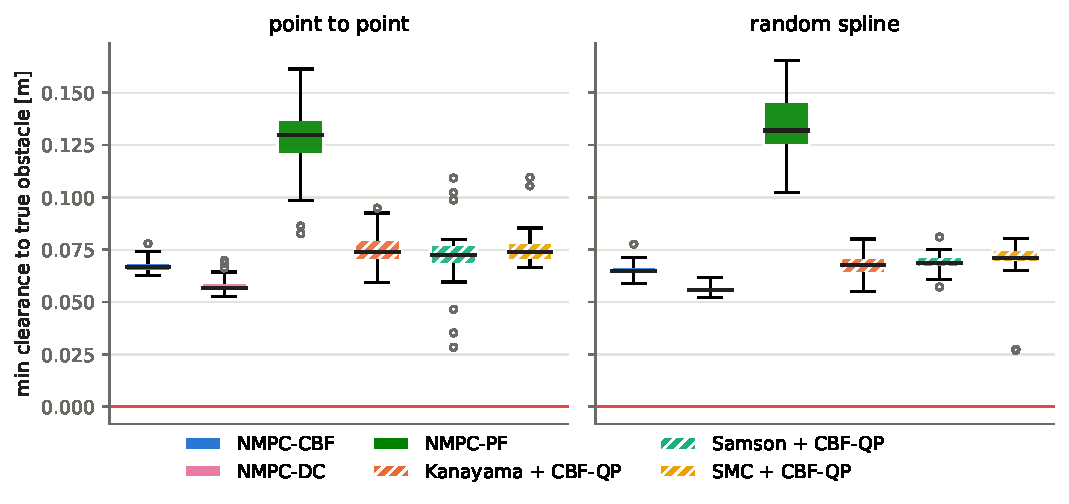
\includegraphics[width=0.85\linewidth]{obstacles_clearance.pdf}\caption{Minimum clearance between robot footprint and true obstacle boundary (hatched: baselines with CBF-QP filter).}\label{fig:obsclear}\end{figure}
\begin{figure}[t]\centering
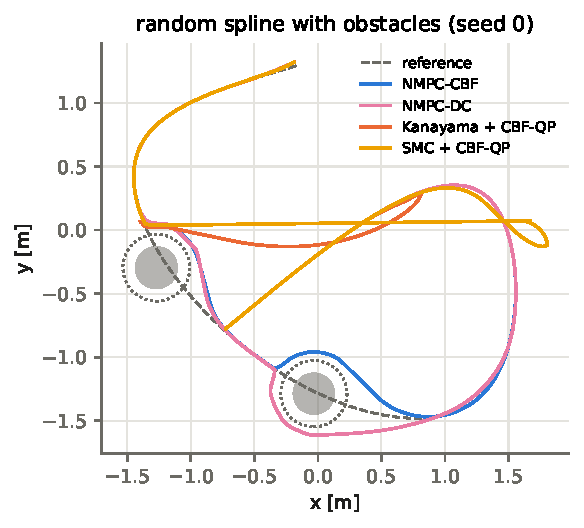
\includegraphics[width=0.49\linewidth]{obstacles_xy_random_spline.pdf}\hfill
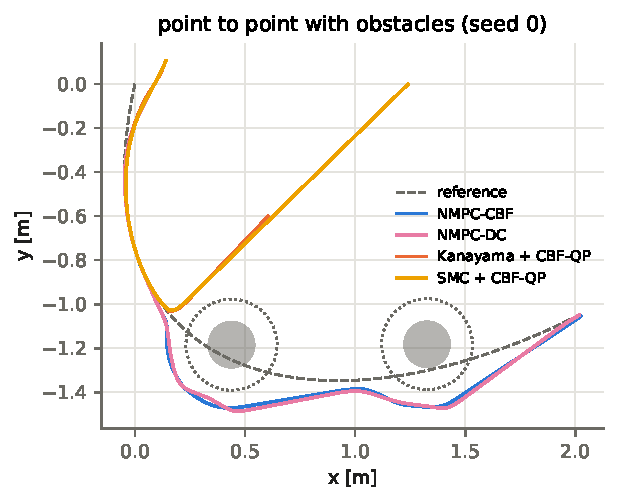
\includegraphics[width=0.49\linewidth]{obstacles_xy_point_to_point.pdf}
\caption{Obstacle scenarios (seed 0). Grey disks: true obstacles; dotted: footprint-inflated boundary.}\label{fig:obsxy}\end{figure}

\subsection{Ablations and computation}
Table~\ref{tab:gamma} reproduces the qualitative finding of~\cite{zeng2021mpccbf} on this robot: smaller $\gamma$ keeps a larger safety margin, and $\gamma=1$ coincides with the distance constraint. Fig.~\ref{fig:ablation} shows that the horizon beyond $N\approx10$ buys little tracking accuracy at the cost of solve time, and Table~\ref{tab:solvetime} that warm-started IPOPT solves the full obstacle problem at $N=20$ with p99 $\approx\SI{21}{ms}$, i.e.\ no missed \SI{100}{ms} deadlines.
\begin{table}[!htbp]
\centering\small
\caption{Obstacle-constraint ablation (point-to-point, 2 obstacles): median clearance, success rate and median per-run p95 solve time. $\gamma=1$ recovers the distance constraint.}\label{tab:gamma}
\begin{adjustbox}{max width=\linewidth}
\begin{tabular}{lrrrrrr}
\toprule
& \multicolumn{3}{c}{$N=10$} & \multicolumn{3}{c}{$N=20$} \\
\cmidrule(lr){2-4}\cmidrule(lr){5-7}
arm & clear. [cm] & succ. [\%] & p95 [ms] & clear. [cm] & succ. [\%] & p95 [ms] \\
\midrule
CBF, $\gamma=0.05$ & 8.0 & 100 & 36.0 & 7.8 & 100 & 71.3 \\
CBF, $\gamma=0.1$ & 4.9 & 100 & 29.7 & 4.9 & 100 & 48.1 \\
CBF, $\gamma=0.2$ & 4.6 & 100 & 29.4 & 4.6 & 100 & 47.2 \\
CBF, $\gamma=0.3$ & 4.5 & 100 & 30.8 & 4.5 & 100 & 52.9 \\
CBF, $\gamma=0.5$ & 4.5 & 100 & 30.7 & 4.5 & 100 & 51.7 \\
CBF, $\gamma=1$ & 4.5 & 100 & 26.3 & 4.5 & 100 & 42.7 \\
DC & 4.5 & 100 & 31.1 & 4.5 & 100 & 41.6 \\
PF & 8.0 & 100 & 15.5 & 9.3 & 100 & 17.6 \\
\bottomrule
\end{tabular}
\end{adjustbox}
\end{table}

\begin{table}[!htbp]
\centering\small
\caption{Warm-started NMPC solve times (IPOPT, serial, Intel i5-1240P); first (cold) solve excluded. Random splines, 2 obstacles for CBF rows.}\label{tab:solvetime}
\begin{adjustbox}{max width=\linewidth}
\begin{tabular}{lrrrrrrrr}
\toprule
configuration & $N$ & solves & mean & median & p95 & p99 & max [ms] & misses [\%] \\
\midrule
NMPC & 20 & 6254 & 2.6 & 2.4 & 3.5 & 4.8 & 9.5 & 0.0 \\
NMPC-CBF & 10 & 6254 & 7.4 & 6.7 & 11.1 & 15.8 & 28.3 & 0.0 \\
NMPC-CBF & 20 & 6254 & 11.2 & 10.1 & 16.1 & 20.8 & 82.2 & 0.0 \\
NMPC-CBF & 30 & 6254 & 14.7 & 13.1 & 21.1 & 24.0 & 41.0 & 0.0 \\
\bottomrule
\end{tabular}
\end{adjustbox}
\end{table}

\begin{figure}[t]\centering
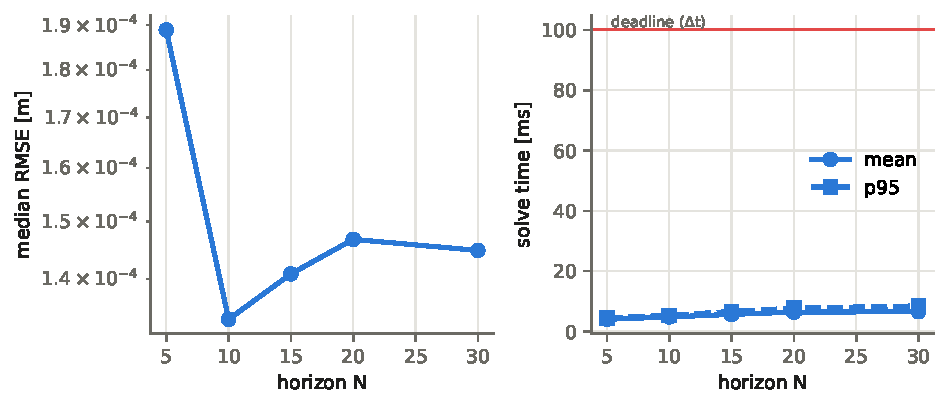
\includegraphics[width=0.49\linewidth]{ablation_horizon.pdf}\hfill
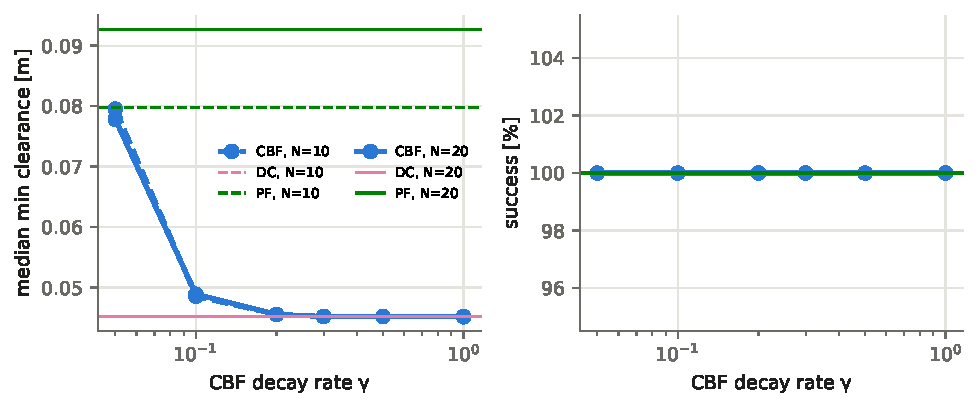
\includegraphics[width=0.49\linewidth]{ablation_gamma.pdf}
\caption{Horizon ablation (left) and obstacle-constraint ablation (right).}\label{fig:ablation}\end{figure}
\begin{figure}[t]\centering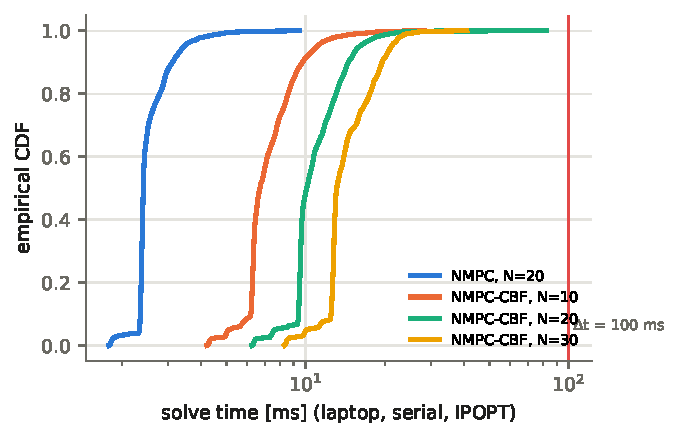
\includegraphics[width=0.6\linewidth]{solve_time_cdf.pdf}\caption{Empirical CDF of warm-started NMPC solve times (serial, laptop CPU).}\label{fig:cdf}\end{figure}

\subsection{Gazebo and hardware}
\begin{figure}[t]\centering
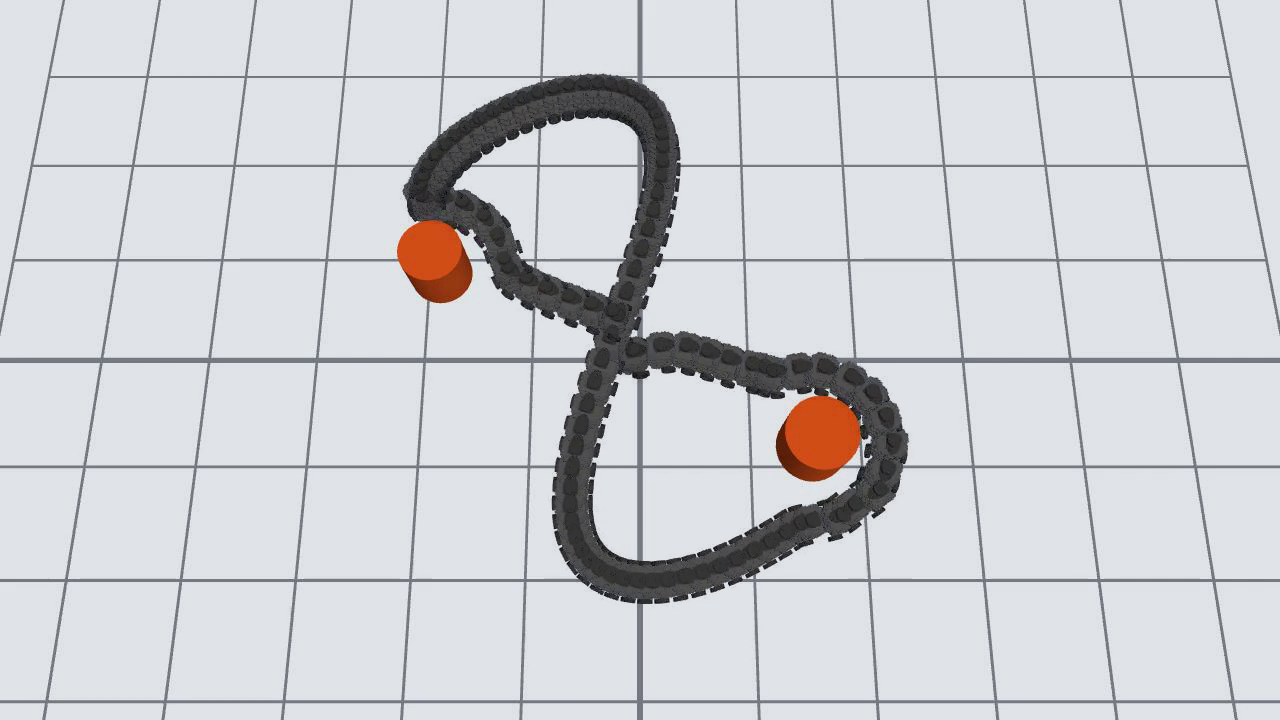
\includegraphics[width=0.49\linewidth]{gazebo_nmpc_figure8.png}\hfill
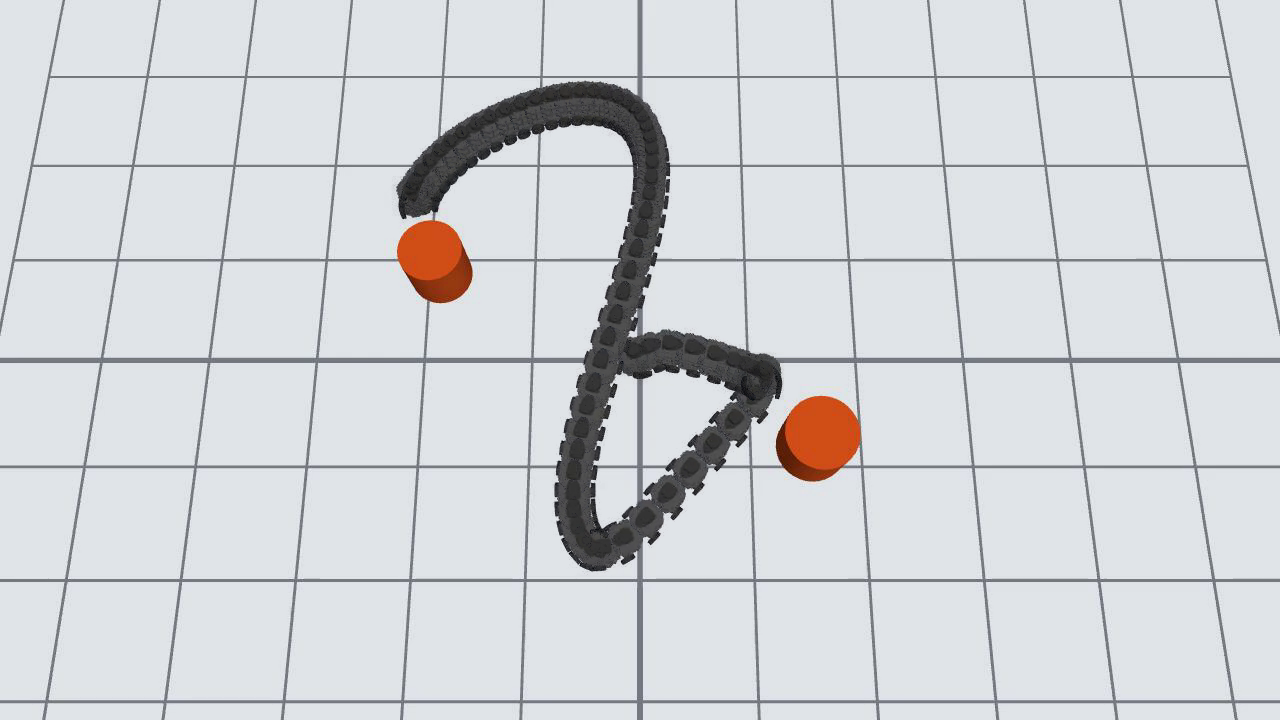
\includegraphics[width=0.49\linewidth]{gazebo_smc_cbfqp_figure8.png}
\caption{Gazebo (encoder odometry, LiDAR obstacle extraction, \SI{10}{Hz} loop): NMPC-CBF (left) and SMC + CBF-QP (right) on the same figure-8 with two obstacles. Videos: \texttt{media/}.}\label{fig:gazebo}\end{figure}
% TODO after lab day: table sim vs Gazebo vs hardware for the same reference; measured /odom and /scan
% rates, step-test dead time (experiments/hw_step_test.py), odometry drift vs tape-measured end pose.

\section{Discussion and limitations}
% Where NMPC wins (preview, constraints, obstacles) and where it does not (model mismatch, compute).
% Obstacle advantage comes from prediction + constraints, not tracking quality.
\paragraph{Trajectory tracking vs path following.} The reference is a function of \emph{time}. After a detour the reference point has moved on, and every tracker (NMPC included) minimizes the current position error by cutting a chord towards it rather than re-tracing the skipped part of the path (visible in \texttt{media/nmpc\_horizon.gif}). When geometric adherence to the path matters more than timing, a path-following formulation (progress variable $s$ as an extra state with $\dot s\ge0$, as in model predictive contouring control) is the natural extension.
% Terminal-set gap vs theory; CBF persistent feasibility is open; static obstacles only;
% odometry-only localization -> drift; LiDAR circle model for walls.

\section{Conclusion}

\bibliographystyle{unsrtnat}
\bibliography{refs}
\end{document}
